% Chapter 4, Topic _Linear Algebra_ Jim Hefferon
%  http://joshua.smcvt.edu/linearalgebra
%  2001-Jun-12
\topic{Geometri Proyektif}
\index{geometri proyektif|(}
Terdapat geometri selain geometri Euklides yang sudah kita kenal.
Salah satunya muncul ketika para seniman mengamati bahwa apa yang dilihat
pengamat belum tentu sama dengan apa yang sebenarnya ada.
Sebagai contoh, berikut karya Leonardo da Vinci,
\textit{Perjamuan Terakhir} (\textit{The Last Supper}).
\index{da Vinci, Leonardo}\index{Perjamuan Terakhir@\textit{Perjamuan Terakhir}}
% From http://upload.wikimedia.org/wikipedia/commons/7/77/DaVinci_LastSupper_high_res_2_nowatmrk.jpg
\begin{center} 
  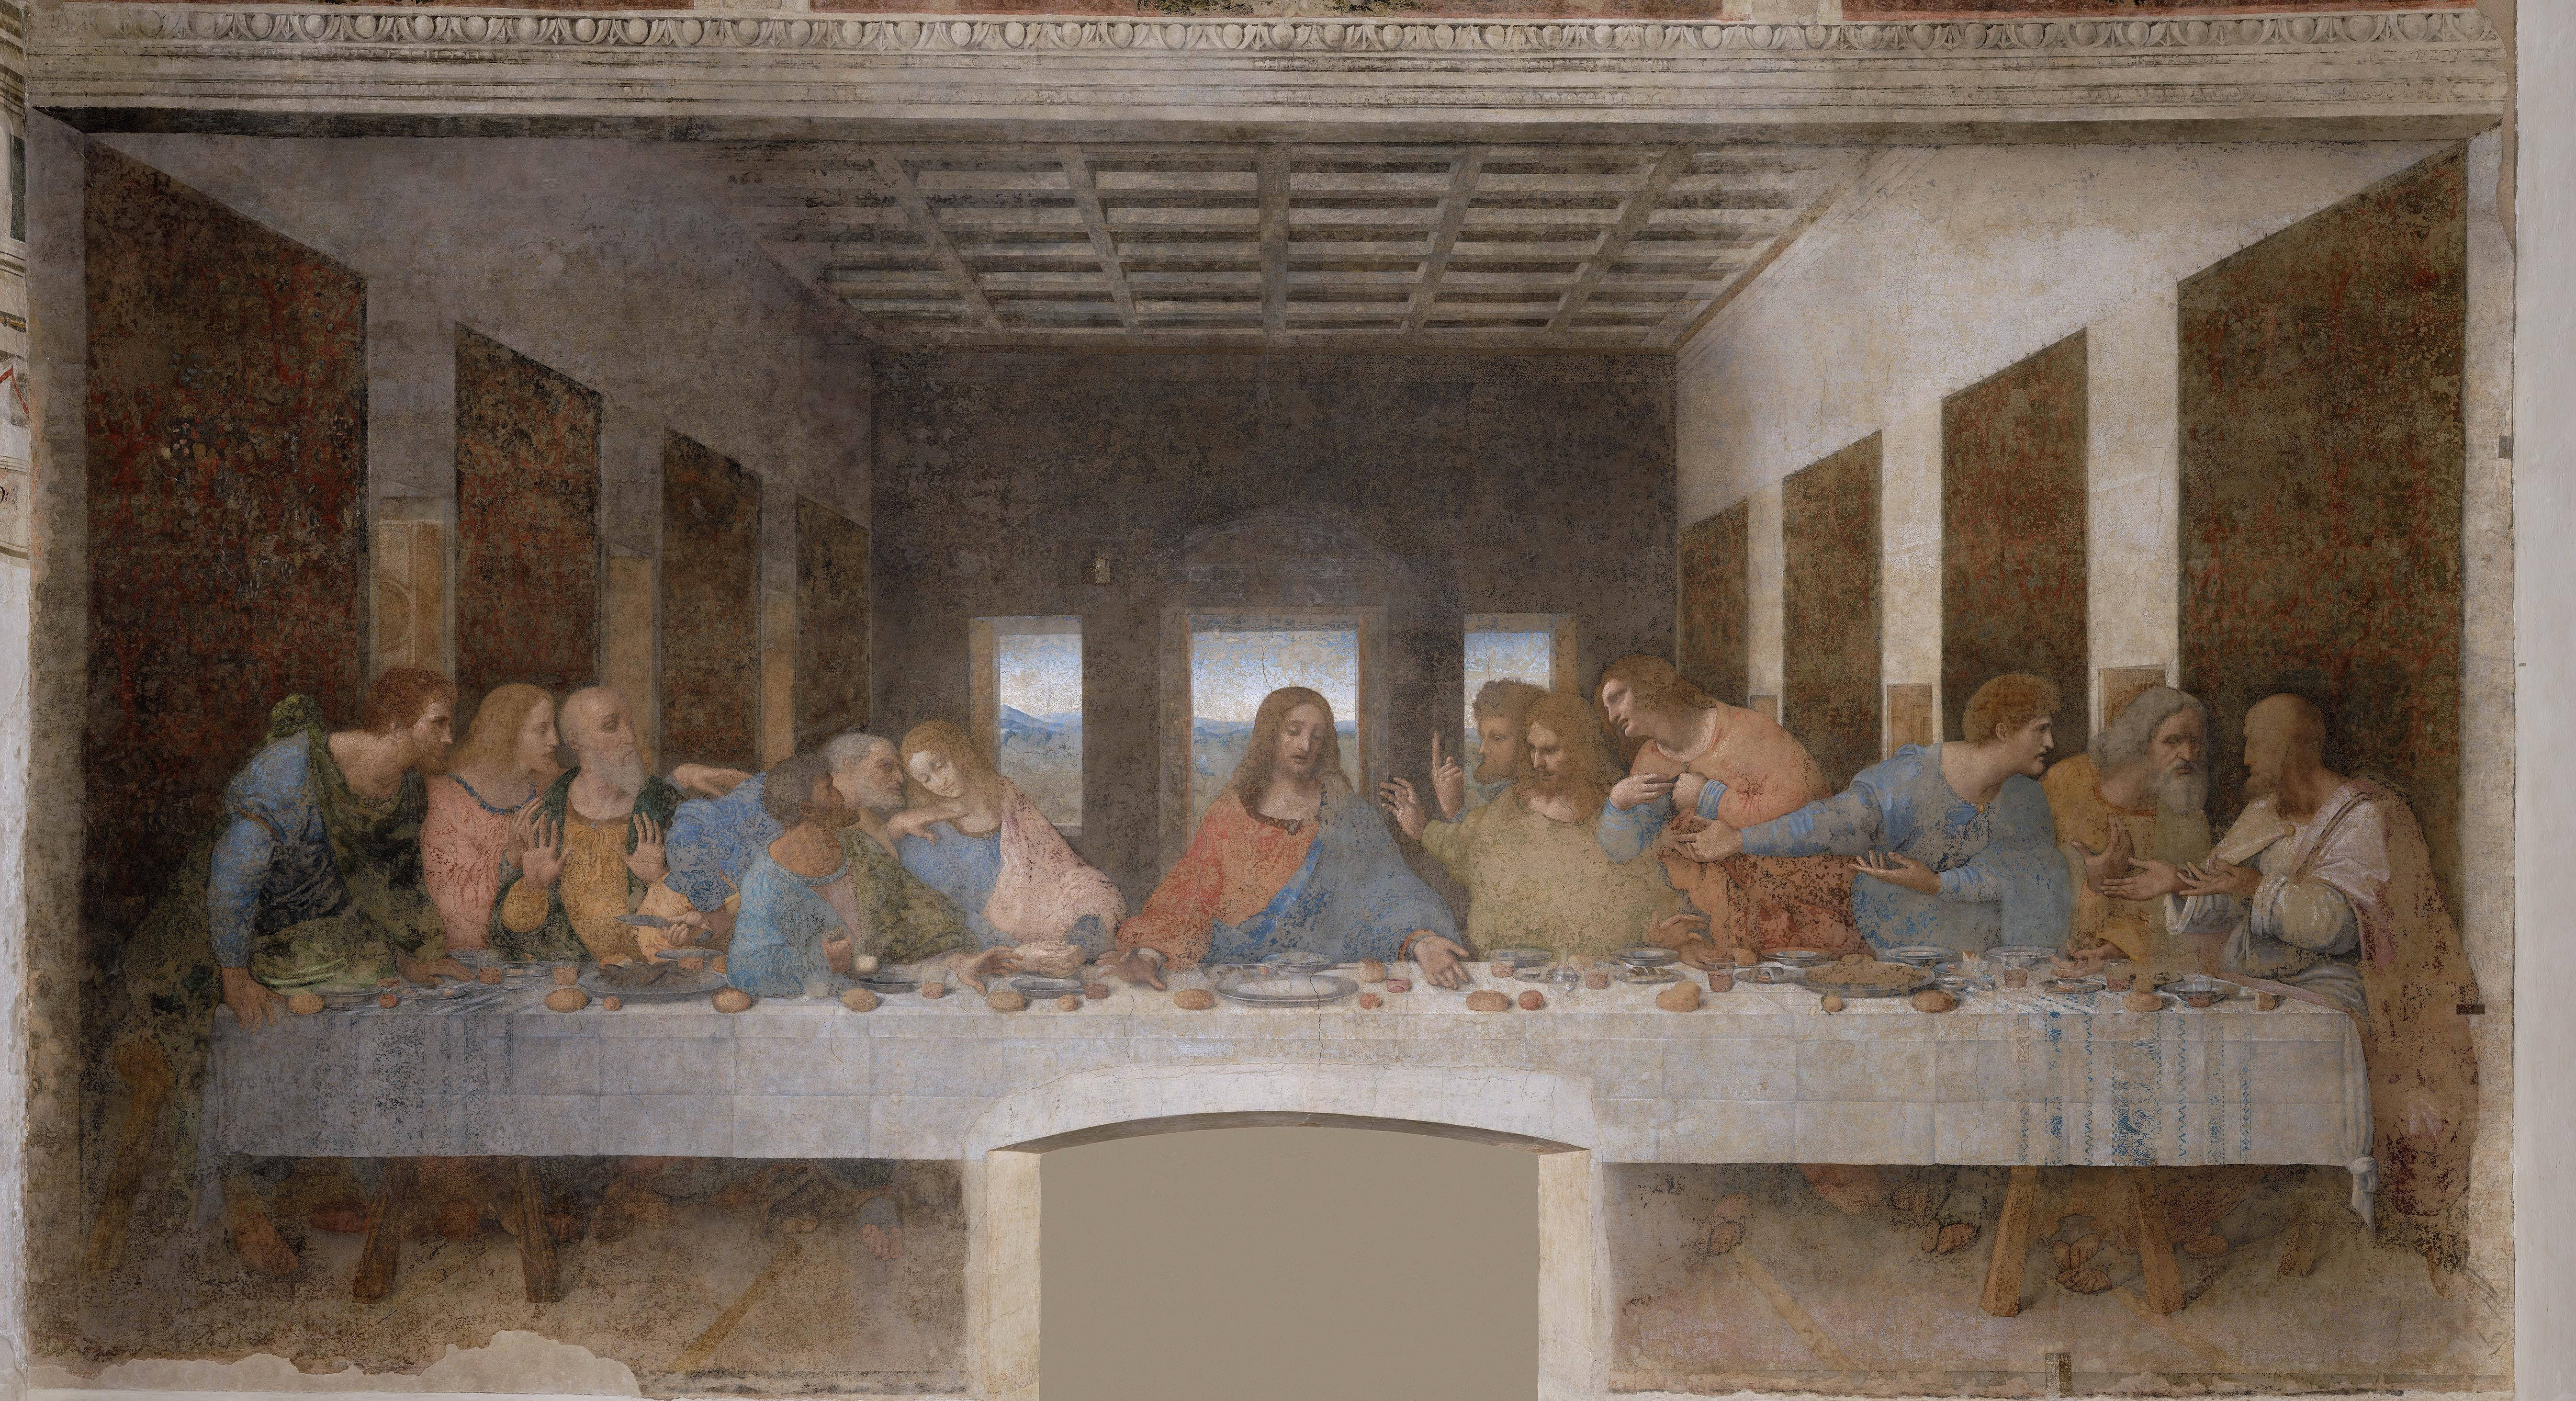
\includegraphics[width=.6\textwidth]{det/pix/LastSupper.jpg}
\end{center}
Perhatikan tempat langit-langit bertemu dinding kiri dan kanan.
Di dalam ruangan, garis-garis tersebut sejajar, tetapi da~Vinci melukiskan
garis-garis yang akan berpotongan jika diperpanjang.
Perpotongan itu disebut \definend{titik hilang}.\index{titik hilang}
\index{proyeksi!pusat!titik hilang}
Aspek perspektif ini kita kenal dari gambar rel kereta yang tampak bertemu di
cakrawala.

Da~Vinci menggunakan suatu model tentang cara kita melihat.
% of how
% we project the three dimensional scene to a two dimensional image.
Bayangkan seseorang sedang memandang sebuah ruangan.
Dari mata orang tersebut, pancarkan sinar ke setiap arah hingga sinar itu
memotong sesuatu, misalnya sebuah titik pada garis pertemuan dinding dan
langit-langit.
Titik potong pertama itulah yang dilihat orang tersebut dalam arah itu.
Secara keseluruhan, yang dilihatnya adalah kumpulan titik potong tiga dimensi
yang diproyeksikan ke suatu gambar dua dimensi bersama.
\begin{center}
  \includegraphics[scale=.8]{det/mp/ch4.5}
\end{center}
Ini adalah \emph{proyeksi pusat}\index{proyeksi!pusat}\index{proyeksi pusat}
dari satu titik.
Seperti ditunjukkan sketsa, proyeksi ini tidak ortogonal seperti proyeksi yang
kita lihat sebelumnya, sebab garis dari pengamat ke~$C$ tidak ortogonal
terhadap bidang gambar.
(Model ini hanya suatu pendekatan\Dash model tidak memperhitungkan faktor
seperti penglihatan binokular atau fakta bahwa pemrosesan oleh otak sangat
memengaruhi persepsi kita.
Meskipun demikian, model ini menarik baik secara artistik maupun matematis.)

Operasi proyeksi pusat mempertahankan sebagian sifat geometris; misalnya, garis
diproyeksikan menjadi garis.
Namun, sebagian sifat lain tidak dipertahankan.
Sebagai contoh, ruas-ruas yang sama panjang dapat diproyeksikan menjadi ruas
dengan panjang yang berbeda (di atas, $AB$ lebih panjang daripada $BC$ karena
ruas yang diproyeksikan ke $AB$ lebih dekat kepada pengamat, dan benda yang
lebih dekat tampak lebih besar).
Kajian tentang efek proyeksi pusat disebut geometri proyektif.

Terdapat tiga kasus proyeksi pusat.
Kasus pertama adalah proyeksi yang dilakukan proyektor film.
\begin{center}
  \includegraphics{det/mp/ch4.6}
\end{center}
Kita dapat membayangkan setiap titik sumber didorong dari bidang domain~$S$ ke
luar menuju bidang gambar~$I$.
Kasus kedua adalah proyeksi seorang seniman yang menarik sumber kembali ke
kanvas.
\begin{center}
  \includegraphics{det/mp/ch4.7}
\end{center}
Kedua kasus ini berbeda karena pada kasus pertama $S$ berada di tengah,
sedangkan pada kasus kedua $I$ berada di tengah.
Masih ada satu konfigurasi lagi, dengan $P$ berada di tengah.
Contohnya adalah ketika kita menggunakan lubang jarum untuk memproyeksikan
gambar gerhana Matahari pada selembar kertas.
\begin{center}
  \includegraphics{det/mp/ch4.8}
\end{center}

Walaupun ketiganya tidak persis sama, ketiganya serupa.
Kita akan menyebut masing-masing sebagai proyeksi pusat oleh $P$ dari $S$
ke~$I$.
Selanjutnya, kita meninjau tiga model proyeksi pusat yang semakin abstrak,
tetapi juga semakin seragam.
Model terakhir akan menonjolkan aljabar linearnya.

%To illustrate some of the geometric effects of these projections,  
Tinjau kembali efek rel kereta yang tampak mengerucut ke satu titik.
Modelkan efek ini dengan garis-garis sejajar pada bidang domain~$S$ dan proyeksi
melalui $P$ ke bidang kodomain~$I$.
(Garis-garis abu-abu yang ditampilkan sejajar dengan bidang~$S$ dan
bidang~$I$.)
\begin{center}
  \includegraphics{det/mp/ch4.9}
\end{center}
Satu konfigurasi ini menunjukkan ketiga kasus proyeksi.
Gambar pertama di bawah menunjukkan $P$ bertindak sebagai proyektor film dengan
mendorong titik-titik dari sebagian $S$ menuju titik-titik gambar pada separuh
bawah~$I$.
Gambar tengah menunjukkan $P$ bertindak sebagai seniman dengan menarik
titik-titik dari bagian lain $S$ kembali ke titik-titik gambar di tengah~$I$.
Pada gambar ketiga, $P$ bertindak sebagai lubang jarum dan memproyeksikan
titik-titik dari $S$ ke bagian atas~$I$.
Gambar ketiga ini paling sulit dipahami\Dash titik-titik yang diproyeksikan dekat
titik hilang adalah titik-titik yang jauh di kiri bawah~$S$.
Titik-titik pada $S$ yang dekat dengan garis abu-abu vertikal dikirim tinggi ke
atas~$I$.
\begin{center}
  \includegraphics{det/mp/ch4.10}
\hfil
  \includegraphics{det/mp/ch4.11}
\hfil
  \includegraphics{det/mp/ch4.12}
\end{center}

Ada dua persoalan di sini.
Pertama, kedua titik dalam domain yang paling dekat dengan garis abu-abu
vertikal (lihat di bawah) tidak memiliki bayangan, sebab proyeksi dari keduanya
berjalan sepanjang garis abu-abu yang sejajar dengan bidang kodomain (kita
mengatakan bahwa kedua titik ini diproyeksikan ke tak hingga).
Kedua, titik hilang pada $I$ bukan bayangan sebarang titik dari $S$, sebab
proyeksi menuju titik itu akan berjalan sepanjang garis abu-abu yang sejajar
dengan bidang domain (kita mengatakan bahwa titik hilang adalah bayangan
proyeksi dari tak hingga).
\begin{center}
  \includegraphics{det/mp/ch4.13}
\end{center}

Untuk memperoleh model yang menghilangkan persoalan tersebut, tutupi proyektor
$P$ dengan kubah setengah bola.
Dalam setiap arah, yang ditentukan oleh suatu garis melalui titik asal,
proyeksikan segala sesuatu dalam arah itu ke satu titik pada kubah tempat garis
tersebut memotongnya.
Ini mencakup proyeksi objek seperti $Q_1$ pada garis di antara $P$ dan kubah,
seperti pada proyektor film.
Ini juga mencakup objek seperti $Q_2$ pada garis yang lebih jauh dari $P$
daripada kubah, seperti pada seniman.
Secara lebih halus, ini juga mencakup objek seperti $Q_3$ yang terletak di
belakang $P$, seperti pada lubang jarum.
\begin{center} 
  \includegraphics{det/mp/ch4.14}
  % \includegraphics{det/mp/ch4.59}
\end{center}
Secara lebih formal, bagi sebarang vektor tak nol $\vec{v}\in\Re^3$, definisikan
\definend{titik $p$ pada bidang proyektif}\index{titik!pada bidang proyektif}
yang terkait sebagai himpunan
$\set{k\vec{v}\suchthat \text{$k\in\Re$ dan $k\neq 0$}}$ dari vektor-vektor tak
nol yang terletak pada garis yang sama melalui titik asal dengan $\vec{v}$.
Untuk mendeskripsikan suatu titik proyektif, kita dapat memberikan sebarang
vektor wakil pada garis tersebut, sehingga titik proyektif yang ditampilkan di
atas dapat direpresentasikan dengan salah satu dari ketiga cara berikut.
\begin{equation*}
  \colvec[r]{1 \\ 2 \\ 3}
  \qquad
  \colvec{1/3 \\ 2/3 \\ 1}
  \qquad
  \colvec[r]{-2 \\ -4 \\ -6}
\end{equation*} 
Masing-masing merupakan \definend{vektor koordinat homogen}
\index{koordinat!homogen}%
\index{vektor koordinat homogen}\index{vektor!koordinat homogen}
bagi titik~$p$.

Gambar dan definisi ini memperjelas proyeksi pusat, tetapi model kubah masih
memiliki suatu kelemahan:~apa yang terjadi ketika $P$ memandang ke bawah?
Pada sketsa di atas, tinjau bagian garis pandang $P$ yang naik menuju kita,
keluar dari halaman.
Bayangkan bagian garis ini turun menuju khatulistiwa dan terus ke bawahnya.
Sekarang bagian garis~$\ell$ yang memotong kubah terletak di belakang halaman.

Artinya, ketika garis pandang terus turun melewati khatulistiwa, titik
proyektif tiba-tiba berpindah dari bagian depan kubah ke bagian belakangnya.
(Hal ini menegaskan bahwa kubah tidak mencakup seluruh khatulistiwa. Jika
mencakup semuanya, ketika pengamat memandang tepat sepanjang khatulistiwa akan
ada dua titik pada garis yang sama-sama berada di kubah.
Sebagai gantinya, kita definisikan kubah agar mencakup titik-titik khatulistiwa
dengan koordinat~$y$ positif, serta titik dengan $y=0$ dan $x$ positif.)
Kelemahan ini berarti kita sering harus memperlakukan titik-titik
khatulistiwa sebagai kasus terpisah.
Jadi, sementara model rel kereta bagi proyeksi pusat memiliki tiga kasus, model
kubah memiliki dua.

Kita dapat memperoleh model yang lebih baik lagi, dengan hanya satu kasus.
Tinjau bola yang berpusat di titik asal.
Setiap garis melalui titik asal memotong bola pada dua titik yang disebut
antipodal.\index{titik antipodal}
Karena kita mengaitkan setiap garis melalui titik asal dengan suatu titik pada
bidang proyektif, kita dapat menggambarkan titik itu sebagai pasangan titik
antipodal pada bola.
Di bawah, kedua titik antipodal dihubungkan oleh garis putus-putus untuk
menegaskan bahwa keduanya bukan dua titik berbeda; pasangan itu bersama-sama
membentuk satu titik proyektif.
\begin{center}
  \includegraphics{det/mp/ch4.15}
\end{center}
Walaupun menggambarkan satu titik sebagai pasangan titik antipodal pada bola
tidak seintuitif model kubah dengan satu titik bagi setiap titik, persoalan pada
model kubah telah hilang:~ketika garis pandang bergeser dari utara ke selatan,
tidak terjadi perubahan mendadak.
Model proyeksi pusat ini seragam.

Sejauh ini, kita telah mendeskripsikan titik-titik dalam geometri proyektif.
Bagaimana dengan garis?
Apa yang dilihat pengamat~$P$ di titik asal sebagai garis ditampilkan di bawah
sebagai lingkaran besar, yaitu perpotongan bola model dengan bidang melalui
titik asal.
\begin{center}
  \includegraphics{det/mp/ch4.16}
\end{center}
(Kita menyertakan salah satu titik proyektif pada garis ini untuk menonjolkan
suatu kehalusan.
Karena dua titik antipodal bersama-sama membentuk satu titik proyektif, bagian
lingkaran besar di belakang halaman merupakan himpunan titik proyektif yang sama
dengan bagian di depan halaman.)
Seperti halnya setiap titik proyektif, kita juga dapat mendeskripsikan garis
proyektif dengan tiga bilangan riil.
Sebagai contoh, anggota-anggota bidang melalui titik asal dalam $\Re^3$ berikut
\begin{equation*}
  %\set{y\colvec[r]{1 \\ -1 \\ 0}+z\colvec[r]{1 \\ 0 \\ 1}\suchthat y,z\in\Re}=
  \set{\colvec{x \\ y \\ z}\suchthat x+y-z=0}
\end{equation*} 
diproyeksikan menjadi garis yang dapat kita deskripsikan dengan
$\rowvec{1 &1 &-1}$ (penggunaan vektor baris membedakan garis dari titik secara
tipografis).
Secara umum, bagi sebarang vektor baris tak nol dengan tiga komponen
$\smash{\vec{L}}$, kita definisikan \definend{garis pada bidang proyektif},
\index{bidang proyektif!garis}\index{garis!pada bidang proyektif}%
yang terkait sebagai himpunan
$L=\set{k\vec{L}\suchthat \text{$k\in\Re$ dan $k\neq 0$}}$.

Deskripsi garis sebagai tiga komponen ini berguna karena pada bidang proyektif,
titik $v$ dan garis $L$ \definend{berinsiden}\Dash titik terletak pada garis
dan garis melalui titik\Dash jika dan hanya jika hasil kali titik wakilnya
$v_1L_1+v_2L_2+v_3L_3$ bernilai nol
(\nearbyexercise{exer:IncidentIndReps} menunjukkan bahwa hal ini tidak
bergantung pada pilihan wakil $\smash{\vec{v}}$ dan $\smash{\vec{L}}$).
Sebagai contoh, titik proyektif yang dideskripsikan di atas oleh vektor kolom
dengan komponen $1$, $2$, dan $3$ terletak pada garis proyektif yang
dideskripsikan oleh $\rowvec{1 &1 &-1}$.
Hal ini terjadi karena sebarang vektor dalam $\Re^3$ yang perbandingan
komponennya $1\mathbin :2\mathbin :3$ terletak pada bidang melalui titik asal
dengan persamaan berbentuk $k\cdot x+k\cdot y-k\cdot z=0$ bagi sebarang
$k\neq0$.
Jadi, rumus insidensi diwarisi dari garis dan bidang ruang tiga dimensi yang
diproyeksikan menjadi $v$ dan $L$.

Dengan ini, kita dapat melakukan geometri proyektif analitik.
Sebagai contoh, garis proyektif $L=\rowvec{1 &1 &-1}$ memiliki persamaan
$1v_1+1v_2-1v_3=0$. Artinya, bagi sebarang titik proyektif~$v$ yang
berinsiden dengan garis tersebut, setiap vektor koordinat homogen wakil $v$
memenuhi persamaan itu.
Hal ini benar karena vektor-vektor tersebut terletak pada bidang dalam ruang
tiga dimensi.
Salah satu perbedaan dari geometri analitik Euklides adalah bahwa dalam
geometri proyektif, selain membicarakan persamaan garis, kita juga membicarakan
persamaan titik.
Bagi titik tetap
\begin{equation*}
  v=\colvec[r]{1 \\ 2 \\ 3}
\end{equation*}
sifat yang mencirikan garis-garis yang berinsiden dengan titik ini adalah bahwa
komponen sebarang wakilnya memenuhi $1L_1+2L_2+3L_3=0$, sehingga inilah
persamaan~$v$.

Kesimetrian pernyataan tentang garis dan titik ini merupakan
\definend{Prinsip Dualitas}\index{Prinsip Dualitas, geometri proyektif}
dalam geometri proyektif:~dalam sebarang pernyataan benar tentang insidensi
pada bidang proyektif, pertukaran `titik' dengan `garis' serta pertukaran
konstruksi penghubungan dengan perpotongan menghasilkan pernyataan benar lain.
Sebagai contoh, sebagaimana dua titik berbeda menentukan tepat satu garis,
dalam bidang proyektif dua garis berbeda menentukan tepat satu titik.
Gambar berikut menunjukkan dua garis proyektif yang berpotongan pada pasangan
titik antipodal dan dengan demikian berpotongan pada satu titik proyektif.
\begin{center}
  \hfill
  \begin{tabular}{@{}c@{}}\includegraphics{det/mp/ch4.17}\end{tabular}
   \hfill\llap{($*$)} 
\end{center}
Bandingkan hal ini dengan geometri Euklides, tempat dua garis berbeda mungkin
memiliki satu titik potong atau mungkin sejajar.
Dalam hal ini, geometri proyektif lebih sederhana dan lebih seragam daripada
geometri Euklides.

Kesederhanaan itu penting karena terdapat hubungan antara kedua ruang:~kita
dapat memandang bidang proyektif sebagai perluasan bidang Euklides.
Gambarkan model bola bagi bidang proyektif sebagai bola satuan dalam $\Re^3$.
Ambil ruang Euklides berdimensi dua sebagai bidang $z=1$.
Seperti ditunjukkan di bawah, semua titik pada bidang Euklides merupakan
proyeksi pasangan titik antipodal dari bola.
Sebaliknya, kita dapat memandang sebagian titik pada bidang proyektif sebagai
titik yang bersesuaian dengan titik dalam ruang Euklides.
(Perhatikan bahwa titik-titik proyektif pada khatulistiwa tidak bersesuaian
dengan titik pada bidang Euklides; kita mengatakan bahwa titik-titik itu
diproyeksikan ke tak hingga.)
\begin{center}
 \hfill
  \begin{tabular}{@{}c@{}}\includegraphics{det/mp/ch4.18}\end{tabular}
 \hfill\llap{($**$)}
\end{center}
Dengan demikian, kita dapat memandang ruang proyektif sebagai bidang Euklides
yang ditambahi beberapa titik\Dash bidang Euklides tertanam dalam bidang
proyektif.
Titik-titik tambahan dalam ruang proyektif, yaitu titik-titik khatulistiwa,
disebut \definend{titik ideal}\index{ideal!titik}%
\index{bidang proyektif!titik ideal} atau
\definend{titik di tak hingga}\index{titik!di tak hingga}, sedangkan
khatulistiwa disebut \definend{garis ideal}\index{ideal!garis}%
\index{bidang proyektif!garis ideal} atau
\definend{garis di tak hingga}\index{garis di tak hingga}
(garis ini bukan garis Euklides, melainkan garis proyektif).

Keuntungan perluasan dari bidang Euklides ke bidang proyektif ini adalah bahwa
sebagian ketidakseragaman geometri Euklides menghilang.
Sebagai contoh, garis-garis proyektif pada~($*$) di atas berpotongan pada
pasangan titik antipodal, yaitu satu titik proyektif.
Jika kita menempatkan garis-garis itu dalam~($**$), garis tersebut bersesuaian
dengan garis-garis Euklides yang sejajar.
Artinya, ketika beralih dari bidang Euklides ke bidang proyektif, kita beralih
dari dua kasus\Dash garis-garis berbeda berpotongan atau sejajar\Dash menjadi
satu kasus saja:~garis-garis berbeda selalu berpotongan (mungkin pada titik di
tak hingga).

Kekurangan bidang proyektif adalah bahwa kita tidak seakrab dengannya seperti
dengan bidang Euklides.
Geometri analitik pada bidang proyektif membantu karena persamaan-persamaannya
mengarahkan kita pada kesimpulan yang tepat.
Geometri proyektif analitik menggunakan aljabar linear.
Sebagai contoh, bagi tiga titik $t$, $u$, dan~$v$ pada bidang proyektif,
penyusunan persamaan titik-titik tersebut dengan menetapkan vektor wakil bagi
masing-masing menunjukkan bahwa ketiganya segaris jika dan hanya jika sistem
tiga persamaan yang dihasilkan memiliki tak hingga banyak solusi vektor baris
yang merepresentasikan garisnya.
Hal itu, pada gilirannya, berlaku jika dan hanya jika determinan berikut nol.
\begin{equation*}
  \begin{vmat}
    t_1  &u_1  &v_1  \\
    t_2  &u_2  &v_2  \\
    t_3  &u_3  &v_3  
  \end{vmat}
\end{equation*}
Jadi, tiga titik pada bidang proyektif segaris jika dan hanya jika tiga vektor
kolom sebarang yang mewakilinya bergantung linear.
Demikian pula, menurut dualitas, tiga garis pada bidang proyektif berinsiden
pada satu titik jika dan hanya jika tiga vektor baris sebarang yang mewakilinya
bergantung linear.

Hasil berikut memberikan bukti tambahan mengenai keteraturan geometri bidang
proyektif. Kita membatasi diri pada konfigurasi tak degenerat:~kedua segitiga
memiliki tiga titik sudut berbeda yang tak segaris, tidak ada tiga di antara
$T_1,U_1,V_1,O$ yang segaris, dan pada setiap garis melalui $O$ kedua titik
sudut yang bersesuaian berbeda satu sama lain dan dari $O$.
Kedua segitiga berikut \definend{berperspektif}
\index{perspektif, segitiga} dari titik $O$ karena pasangan titik sudut yang
bersesuaian terletak pada satu garis.
\begin{center}
  \includegraphics{det/mp/ch4.19}
\end{center}
Tinjau pasangan sisi yang bersesuaian:~sisi $T_1U_1$ dan $T_2U_2$, sisi
$T_1V_1$ dan $T_2V_2$, serta sisi $U_1V_1$ dan $U_2V_2$.
\definend{Teorema Desargues}\index{Teorema Desargues}
menyatakan bahwa ketika ketiga pasangan sisi yang bersesuaian diperpanjang,
pasangan-pasangan itu berpotongan (ditampilkan di sini sebagai titik $TU$,
$TV$, dan $UV$).
Lebih lanjut, ketiga titik potong tersebut segaris.
\begin{center}
  \includegraphics{det/mp/ch4.23}
\end{center}
Kita akan membuktikannya menggunakan geometri proyektif.
(Kita menggambar bangun Euklides karena gambar tersebut lebih dikenal.
Untuk memandangnya sebagai bangun proyektif, kita dapat membayangkan bahwa
walaupun ruas-ruas garis yang ditampilkan merupakan bagian lingkaran besar dan
karena itu melengkung, jari-jari model sangat besar dibandingkan ukuran bangun
sehingga sisi-sisinya tampak lurus pada sketsa.)

Untuk pembuktian, kita memerlukan lema pendahuluan \cite{Coxeter}:~jika $W$,
$X$, $Y$, dan $Z$ merupakan empat titik pada bidang proyektif dan tidak ada
tiga di antaranya yang segaris, maka terdapat vektor koordinat homogen
$\vec{w}$, $\vec{x}$, $\vec{y}$, dan $\vec{z}$ bagi titik-titik proyektif
tersebut, serta basis $B$ bagi $\Re^3$, yang memenuhi
\begin{equation*}
  \rep{\vec{w}}{B}=\colvec[r]{1 \\ 0 \\ 0}
  \quad
  \rep{\vec{x}}{B}=\colvec[r]{0 \\ 1 \\ 0}
  \quad
  \rep{\vec{y}}{B}=\colvec[r]{0 \\ 0 \\ 1}
  \quad
  \rep{\vec{z}}{B}=\colvec[r]{1 \\ 1 \\ 1}
\end{equation*}
Untuk membuktikan lema tersebut, karena $W$, $X$, dan $Y$ tidak terletak pada
garis proyektif yang sama, sebarang vektor koordinat homogen
$\vec{w}_0$, $\vec{x}_0$, dan $\vec{y}_0$ tidak terletak pada bidang yang sama
melalui titik asal dalam $\Re^3$, sehingga membentuk himpunan perentang
bagi~$\Re^3$.
Karena itu, sebarang vektor koordinat homogen bagi $Z$ merupakan kombinasi
$\vec{z}_0=a\cdot\vec{w}_0+b\cdot\vec{x}_0+c\cdot\vec{y}_0$.
Syarat bahwa tidak ada tiga titik yang segaris memastikan
$a,b,c\neq0$.
Ambil $B=\sequence{\vec{w},\vec{x},\vec{y}}$ sebagai basis, dengan
$\vec{w}=a\cdot\vec{w}_0$, $\vec{x}=b\cdot\vec{x}_0$,
$\vec{y}=c\cdot\vec{y}_0$, dan $\vec{z}=\vec{z}_0$.

Untuk membuktikan Teorema Desargues, gunakan lema tersebut untuk menetapkan
vektor koordinat homogen dan suatu basis.
\begin{equation*}
  \rep{\vec{t}_1}{B}=\colvec[r]{1 \\ 0 \\ 0}
  \quad
  \rep{\vec{u}_1}{B}=\colvec[r]{0 \\ 1 \\ 0}
  \quad
  \rep{\vec{v}_1}{B}=\colvec[r]{0 \\ 0 \\ 1}
  \quad
  \rep{\vec{o}}{B}=\colvec[r]{1 \\ 1 \\ 1}    
\end{equation*}
Titik proyektif $T_2$ berinsiden dengan garis proyektif $OT_1$, sehingga
sebarang vektor koordinat homogen bagi $T_2$ terletak pada bidang melalui titik
asal dalam $\Re^3$ yang direntang oleh vektor koordinat homogen $O$ dan $T_1$:
\begin{equation*}
  \rep{\vec{t}_2}{B}=a\colvec[r]{1 \\ 1 \\ 1}
                          +b\colvec[r]{1 \\ 0 \\ 0}
\end{equation*}
untuk suatu skalar $a$ dan $b$.
Jadi, vektor koordinat homogen titik $T_2$ pada garis $OT_1$ memiliki bentuk
paling kiri di bawah.
Bentuk bagi $U_2$ dan $V_2$ serupa.
\begin{equation*}
  \rep{\vec{t}_2}{B}=\colvec{t_2 \\ 1 \\ 1}
  \qquad
  \rep{\vec{u}_2}{B}=\colvec{1 \\ u_2 \\ 1}
  \qquad
  \rep{\vec{v}_2}{B}=\colvec{1 \\ 1 \\ v_2}
\end{equation*}
Garis proyektif $T_1U_1$ merupakan proyeksi suatu bidang melalui titik asal
dalam $\Re^3$.
Salah satu cara memperoleh persamaannya adalah dengan memperhatikan bahwa
sebarang vektor di dalamnya bergantung linear pada vektor bagi $T_1$ dan $U_1$,
sehingga determinan berikut nol.
\begin{equation*}
  \begin{vmat}
    1  &0  &x  \\
    0  &1  &y  \\
    0  &0  &z
  \end{vmat}=0
  \qquad
  \Longrightarrow
  \qquad
  z=0
\end{equation*}
Persamaan bidang dalam $\Re^3$ yang bayangannya merupakan garis proyektif
$T_2U_2$ adalah
\begin{equation*}
  \begin{vmat}
    t_2  &1    &x  \\
    1    &u_2  &y  \\
    1    &1    &z
  \end{vmat}=0
  \qquad
  \Longrightarrow
  \qquad
  (1-u_2)\cdot x+(1-t_2)\cdot y+(t_2u_2-1)\cdot z=0
\end{equation*}
Mencari perpotongan keduanya merupakan perhitungan rutin.
\begin{equation*}
  T_1U_1\,\intersection\, T_2U_2
  =\colvec{t_2-1 \\ 1-u_2 \\ 0}
\end{equation*}
(Tentu saja, ini merupakan vektor koordinat homogen suatu titik proyektif.)
Kedua perpotongan lainnya diperoleh secara serupa.
\begin{equation*}
  T_1V_1\,\intersection\, T_2V_2
  =\colvec{1-t_2 \\ 0 \\ v_2-1}
  \qquad
  U_1V_1\,\intersection\, U_2V_2
  =\colvec{0 \\ u_2-1 \\ 1-v_2}
\end{equation*}
Selesaikan pembuktian dengan memperhatikan bahwa titik-titik proyektif ini
terletak pada satu garis proyektif karena jumlah ketiga vektor koordinat
homogennya adalah nol.

Setiap teorema proyektif memiliki padanan dalam versi Euklides, walaupun hasil
Euklidesnya mungkin lebih rumit untuk dinyatakan dan dibuktikan.
Teorema Desargues menggambarkan hal ini.
Dalam padanan ruang Euklides, kita harus menangani secara terpisah kasus ketika
$O$ terletak pada garis ideal, sebab garis $T_1T_2$, $U_1U_2$, dan $V_1V_2$
menjadi sejajar.

Catatan setelah pernyataan Teorema Desargues menyarankan agar kita memandang
gambar Euklides sebagai bangun geometri proyektif dalam model bola berjari-jari
sangat besar.
Artinya, seperti sebagian kecil permukaan dunia tampak datar bagi orang yang
tinggal di sana, bidang proyektif bersifat Euklides secara lokal.

Kita menutup topik ini dengan mendeskripsikan satu hal lagi tentang bidang
proyektif.
Walaupun sifat lokalnya sudah kita kenal, bidang proyektif memiliki sifat global
yang mungkin terasa asing.
Gambar di bawah menunjukkan suatu titik proyektif.
Seperti dijelaskan di atas, titik itu terdiri atas dua titik antipodal,
$Q_1$ dan~$Q_2$, tetapi keduanya merupakan satu titik dalam bidang proyektif.
Pada titik tersebut, kita menggambar sumbu Kartesius, yaitu sumbu~$xy$.
Sumbu-sumbu ini tampak pada kedua titik antipodal dalam gambar, satu di belahan
utara pada $Q_1$ dan satu lagi di selatan pada~$Q_2$.
Perhatikan bahwa pada belahan utara, sumbu~$x$ positif menunjuk ke kanan.
Artinya, seseorang yang menaruh tangan kanan pada bola dengan telapak menghadap
ke bawah dan ibu jari pada sumbu~$y$ akan memiliki jari-jari yang menunjuk
searah sumbu~$x$ positif.
% But the antipodal axes give the opposite:~if a person puts their
% right hand on the southern hemisphere spot on the sphere,  palm on the 
% sphere's surface, 
% with their fingers pointing toward positive infinity on the $x$-axis, then
% their thumb points on the $y$-axis toward negative infinity.
% Instead, 
% to have their fingers point positively on the $x$-axis and their thumb
% point positively on the $y$, a person must use their left hand.
% Briefly, the projective plane is not orientable\Dash in this geometry,
% left and right handedness are not fixed properties of figures.
\begin{center}
  \includegraphics{det/mp/ch4.24}
\end{center}
Urutan gambar di bawah menunjukkan perjalanan mengelilingi ruang ini sepanjang
garis proyektif:~$Q_1$ bergerak naik melewati kutub utara dan berakhir pada sisi
jauh bola, sedangkan pasangannya~$Q_2$ bergerak ke depan.
(Hati-hati:~perjalanan ini bukan hanya setengah putaran mengelilingi bidang
proyektif, melainkan satu putaran penuh.
Titik-titik antipodal pada kedua ujung garis putus-putus membentuk satu titik
proyektif.
Karena itu, pada gambar ketiga perjalanan telah kembali ke titik proyektif yang
pada dasarnya sama dengan titik awalnya.)
\begin{center}
  \begin{tabular}{@{}c@{}}\includegraphics{det/mp/ch4.25}\end{tabular}
\qquad\mbox{$\Longrightarrow$}\qquad
  \begin{tabular}{@{}c@{}}\includegraphics{det/mp/ch4.26}\end{tabular}
\qquad\mbox{$\Longrightarrow$}\qquad
  \begin{tabular}{@{}c@{}}\includegraphics{det/mp/ch4.27}\end{tabular}
\end{center}
Pada akhir putaran, bagian~$x$ dari sumbu~$xy$ menunjuk ke arah yang
berlawanan.
Artinya, agar seseorang dapat meletakkan ibu jari pada sumbu~$y$ dan
jari-jarinya menunjuk ke arah positif sumbu~$x$, ia harus menggunakan tangan
kiri.
Bidang proyektif tidak dapat diorientasikan\Dash dalam geometri ini, sifat
bertangan kiri atau bertangan kanan bukan sifat tetap suatu bangun.
Sebagai contoh, kita tidak dapat mendeskripsikan spiral sebagai berarah jarum
jam atau berlawanan arah jarum jam.

Contoh keberadaan ruang yang tidak dapat diorientasikan ini menimbulkan
pertanyaan apakah alam semesta kita dapat diorientasikan.
Mungkinkah seorang astronaut meninggalkan Bumi dengan orientasi tangan kanan
dan kembali dengan orientasi tangan kiri?
\cite{Gardner} merupakan rujukan nonteknis.
\cite{Clarke} merupakan cerita fiksi ilmiah klasik tentang pembalikan orientasi.

Untuk ikhtisar geometri proyektif, lihat \cite{CourantRobbins}.
Pendekatan yang kita gunakan di sini, yaitu pendekatan analitik, menghasilkan
teorema dengan cepat dan % \Dash  most importantly for us \Dash 
menunjukkan kekuatan aljabar linear; lihat \cite{Hanes}, \cite{Ryan}, dan
\cite{Eggar}.
Namun, pendekatan lain, yaitu pendekatan sintetis yang menurunkan hasil dari
suatu sistem aksioma, luar biasa indah dan juga merupakan jalur perkembangan
historisnya.
Dua sumber yang baik untuk pendekatan ini adalah \cite{Coxeter} dan
\cite{Seidenberg}.
Penerapan yang mudah dan menarik terdapat dalam \cite{Davies}.

\begin{exercises}
  \item 
    Tentukan persamaan titik berikut.
    \begin{equation*}
       \colvec[r]{1 \\ 0 \\ 0}
    \end{equation*}
    \begin{answer}
      Dari hasil kali titik
      \begin{equation*}
        0=\colvec[r]{1 \\ 0 \\ 0}\dotprod\rowvec{L_1 &L_2 &L_3}
         =L_1
      \end{equation*}
      kita memperoleh persamaan $L_1=0$.
    \end{answer}
  \item 
    \begin{exparts}
      \partsitem Cari garis yang berinsiden dengan titik-titik berikut pada
         bidang proyektif.
         \begin{equation*}
           \colvec[r]{1 \\ 2 \\ 3},\,\colvec[r]{4 \\ 5 \\ 6}
         \end{equation*}
      \partsitem Cari titik yang berinsiden dengan kedua garis proyektif berikut.
         \begin{equation*}
           \rowvec{1 &2 &3},\,\rowvec{4 &5 &6}
         \end{equation*} 
    \end{exparts}
    \begin{answer}
      \begin{exparts}
        \partsitem Determinan berikut
          \begin{equation*}
            0=\begin{vmat}
              1  &4  &x \\
              2  &5  &y \\
              3  &6  &z
            \end{vmat}
            =-3x+6y-3z
          \end{equation*}
          menunjukkan bahwa garisnya adalah $L=\rowvec{-3 &6 &-3}$.
        \partsitem $\colvec[r]{-3 \\ 6 \\ -3}$
      \end{exparts}
    \end{answer}
  \item
    Cari rumus bagi garis yang berinsiden dengan dua titik proyektif.
    Cari rumus bagi titik yang berinsiden dengan dua garis proyektif.
    \begin{answer}
      Garis yang berinsiden dengan
      \begin{equation*}
        u=\colvec{u_1 \\ u_2 \\ u_3}
        \qquad
        v=\colvec{v_1 \\ v_2 \\ v_3}
      \end{equation*}
      diperoleh dari persamaan determinan berikut.
      \begin{equation*}
        0=\begin{vmat}
          u_1  &v_1  &x  \\
          u_2  &v_2  &y  \\
          u_3  &v_3  &z
        \end{vmat}
        =(u_2v_3-u_3v_2)\cdot x 
          + (u_3v_1-u_1v_3)\cdot y 
          + (u_1v_2-u_2v_1)\cdot z
      \end{equation*}
      Rumus bagi titik yang berinsiden dengan dua garis berbentuk sama.
    \end{answer}
  \item \label{exer:IncidentIndReps}
    Buktikan bahwa definisi insidensi tidak bergantung pada pilihan wakil $p$
    dan $L$.
    Artinya, jika $p_1$, $p_2$, $p_3$ dan $q_1$, $q_2$, $q_3$ merupakan dua
    rangkap tiga koordinat homogen bagi $p$, sedangkan $L_1$, $L_2$, $L_3$ dan
    $M_1$, $M_2$, $M_3$ merupakan dua rangkap tiga koordinat homogen bagi $L$,
    buktikan bahwa
    $p_1L_1+p_2L_2+p_3L_3=0$ jika dan hanya jika
    $q_1M_1+q_2M_2+q_3M_3=0$. 
    \begin{answer}
      Karena kedua rangkap tiga bagi $p$ merupakan koordinat homogen bagi titik
      yang sama, kedua vektor kolomnya sebanding, yaitu terletak pada garis yang
      sama melalui titik asal.
      Demikian pula, kedua vektor barisnya sebanding.
      \begin{equation*}
        k\cdot\colvec{p_1 \\ p_2 \\ p_3}
          =\colvec{q_1 \\ q_2 \\ q_3}
        \qquad
        m\cdot\rowvec{L_1 &L_2 &L_3}
          =\rowvec{M_1 &M_2 &M_3}
      \end{equation*}
      Skalar $k$ dan $m$ tidak nol. Karena itu,
      $q_1M_1+q_2M_2+q_3M_3
        =(km)\cdot(p_1L_1+p_2L_2+p_3L_3)$,
      sehingga ruas kiri bernilai nol jika dan hanya jika ekspresi di dalam
      tanda kurung bernilai nol.
    \end{answer}
  \item 
    Berikan gambar yang menunjukkan bahwa proyeksi pusat tidak mempertahankan
    lingkaran, yaitu bahwa lingkaran dapat diproyeksikan menjadi elips.
    Dapatkah elips (yang bukan lingkaran) diproyeksikan menjadi lingkaran?
    %Must it (in the sense that for any ellipse there is a projection
    %such that it would project to a circle)? 
    \begin{answer}
      Gambar gerhana Matahari\Dash kecuali bidang gambar tepat tegak lurus
      terhadap garis dari Matahari melalui lubang jarum\Dash menunjukkan
      lingkaran Matahari diproyeksikan menjadi gambar berbentuk elips.
      (Contoh lain adalah bahwa dalam banyak gambar pada topik ini, kita
      menampilkan lingkaran khatulistiwa bola sebagai elips; pengamat gambar
      melihat suatu lingkaran sebagai elips.)
      
      Gambar gerhana Matahari juga menunjukkan kebalikannya.
      Jika kita membayangkan proyeksi berjalan dari kiri ke kanan melalui lubang
      jarum, elips $I$ diproyeksikan melalui $P$ menjadi lingkaran~$S$.
    \end{answer}
  \item \label{exer:CorrProjPlaneEucPl} 
    Berikan rumus bagi korespondensi antara bagian di luar khatulistiwa dari
    model antipodal bidang proyektif dan bidang $z=1$.
    \begin{answer}
      Suatu titik pada bola satuan
      \begin{equation*}
        \colvec{p_1 \\ p_2 \\ p_3} 
      \end{equation*}
      bukan titik khatulistiwa jika dan hanya jika $p_3\neq 0$.
      Dalam kasus itu, titik tersebut bersesuaian dengan titik berikut pada
      bidang $z=1$:
      \begin{equation*}
        \colvec{p_1/p_3 \\ p_2/p_3  \\ 1}
      \end{equation*}
      sebab titik itu merupakan perpotongan garis yang memuat vektor tersebut
      dengan bidang.
    \end{answer}
%  \item \label{exer:ELinesCorrPLines} 
%    Consider the correspondence between the non-ideal points in
%    the projective plane and the Euclidean plane.
%    \begin{exparts}
%      \item Show that any Euclidean line corresponds to a projective line.
%      \item Show that parallel Euclidean lines correspond to projective
%        lines that meet at an ideal point.
%      \item Prove the converses of those two statements.
%    \end{exparts}
%  \item \label{exer:EuclidDesarg}
%    Give a statement of Desargue's Theorem for Euclidean geometry.
%  \item  \label{exer:DesarAntipPict}
%    Draw a picture illustrating Desargue's Theorem on the antipodal model. 
  \item 
    (Teorema Pappus)
    Andaikan $T_0$, $U_0$, dan $V_0$ merupakan tiga titik berbeda pada satu
    garis, sedangkan $T_1$, $U_1$, dan $V_1$ merupakan tiga titik berbeda pada
    garis lain. Andaikan pula semua perpotongan di bawah terdefinisi dan
    berbeda dari titik-titik yang membentuk garisnya, serta tidak ada tiga di
    antara $T_0,T_1,T_2,V_0$ yang segaris.
    Tinjau tiga titik berikut:
    (i)~perpotongan $V_2$ antara garis $T_0U_1$ dan $T_1U_0$,
    (ii)~perpotongan $U_2$ antara garis $T_0V_1$ dan $T_1V_0$, serta
    (iii)~perpotongan $T_2$ antara $U_0V_1$ dan $U_1V_0$.
    \begin{exparts}
      \partsitem Gambarkan bangun (Euklides).
      \partsitem Terapkan lema yang digunakan dalam Teorema Desargues untuk
        memperoleh vektor koordinat homogen sederhana bagi titik-titik $T$ dan
        $V_0$.
      \partsitem Cari vektor koordinat homogen yang dihasilkan bagi
        titik-titik $U$ (masing-masing harus melibatkan satu parameter; misalnya,
        $U_0$ dapat berada di mana saja pada garis $T_0V_0$).
      \partsitem Cari vektor koordinat homogen yang dihasilkan bagi $V_1$.
        (\textit{Petunjuk:}~vektor ini melibatkan dua parameter.)
      \partsitem Cari vektor koordinat homogen yang dihasilkan bagi $V_2$.
        (Vektor ini juga melibatkan dua parameter.)
      \partsitem Tunjukkan bahwa hasil kali ketiga parameter adalah $1$.
      \partsitem Verifikasi bahwa $V_2$ terletak pada garis $T_2U_2$.
    \end{exparts}
    \begin{answer}
      \begin{exparts}
        \partsitem Gambar lain juga mungkin; berikut salah satunya.
          \begin{center}
            \includegraphics{det/mp/ch4.54}
          \end{center}
          Perpotongan
          $
              T_0U_1\,\intersection T_1U_0=V_2
          $, $
              T_0V_1\,\intersection T_1V_0=U_2
          $, dan $
              U_0V_1\,\intersection U_1V_0=T_2
          $
          diberi label sedemikian sehingga pada setiap garis terdapat satu
          titik $T$, satu titik $U$, dan satu titik $V$.
        \partsitem Lema yang digunakan dalam Teorema Desargues memberikan basis
          $B$ yang terhadapnya titik-titik tersebut memiliki vektor koordinat
          homogen berikut.
          \begin{equation*}
            \rep{\vec{t}_0}{B}=\colvec[r]{1 \\ 0 \\ 0}
            \quad
            \rep{\vec{t}_1}{B}=\colvec[r]{0 \\ 1 \\ 0}
            \quad
            \rep{\vec{t}_2}{B}=\colvec[r]{0 \\ 0 \\ 1}
            \quad
            \rep{\vec{v}_0}{B}=\colvec[r]{1 \\ 1 \\ 1}
          \end{equation*}
        \partsitem
          Pertama, sebarang $U_0$ pada $T_0V_0$
          \begin{equation*}
            \rep{\vec{u}_0}{B}=a\colvec[r]{1 \\ 0 \\ 0}
                               +b\colvec[r]{1 \\ 1 \\ 1}
                              =\colvec{a+b \\ b \\ b}
          \end{equation*}
          memiliki vektor koordinat homogen berbentuk
          \begin{equation*}
            \colvec{u_0 \\ 1 \\ 1}      
          \end{equation*}
          ($u_0$ merupakan parameter; nilainya bergantung pada letak titik $U_0$
          pada garis $T_0V_0$, tetapi setiap titik pada garis tersebut memiliki
          vektor koordinat homogen berbentuk demikian untuk suatu $u_0\in\Re$).
          Demikian pula, $U_2$ terletak pada $T_1V_0$,
          \begin{equation*}
            \rep{\vec{u}_2}{B}=c\colvec[r]{0 \\ 1 \\ 0}
                                +d\colvec[r]{1 \\ 1 \\ 1}
                              =\colvec{d \\ c+d \\ d}
          \end{equation*}
          sehingga memiliki vektor koordinat homogen berikut.
          \begin{equation*}
            \colvec{1 \\ u_2 \\ 1}
          \end{equation*}
          Dengan cara serupa, $U_1$ berinsiden dengan $T_2V_0$,
          \begin{equation*}
            \rep{\vec{u}_1}{B}=e\colvec[r]{0 \\ 0 \\ 1}
                                +f\colvec[r]{1 \\ 1 \\ 1}
                              =\colvec{f \\ f \\ e+f}  
          \end{equation*}
          dan memiliki vektor koordinat homogen berikut.
          \begin{equation*}
            \colvec{1 \\ 1 \\ u_1}
          \end{equation*}
        \partsitem
          Karena $V_1=T_0U_2\,\intersection\,U_0T_2$, kita memiliki
          \begin{equation*}
            g\colvec[r]{1 \\ 0 \\ 0}+h\colvec{1 \\ u_2 \\ 1}
            =i\colvec{u_0 \\ 1 \\ 1}+j\colvec[r]{0 \\ 0 \\ 1}
            \qquad\Longrightarrow\qquad
            \begin{aligned}
              g+h  &= iu_0 \\
              hu_2 &= i    \\
              h    &= i+j
            \end{aligned}
          \end{equation*}
          Substitusi $hu_2$ bagi $i$ dalam persamaan pertama,
          \begin{equation*}
            \colvec{hu_0u_2 \\ hu_2 \\ h}
          \end{equation*}
           menunjukkan bahwa $V_1$ memiliki vektor koordinat homogen dengan
           dua parameter berikut.
          \begin{equation*}
            \colvec{u_0u_2 \\ u_2 \\ 1}
          \end{equation*}
        \partsitem
           Karena $V_2$ merupakan perpotongan
           $T_0U_1\,\intersection\,T_1U_0$,
           \begin{equation*}
             k\colvec[r]{1 \\ 0 \\ 0}+l\colvec{1 \\ 1 \\ u_1}
              =m\colvec[r]{0 \\ 1 \\ 0}+n\colvec{u_0 \\ 1 \\ 1}
            \qquad\Longrightarrow\qquad
            \begin{aligned}
              k+l  &= nu_0 \\
              l    &= m+n    \\
              lu_1 &= n
            \end{aligned}
           \end{equation*}
           dan substitusi $lu_1$ bagi $n$ dalam persamaan pertama,
           \begin{equation*}
             \colvec{lu_0u_1 \\ l \\ lu_1}
           \end{equation*}
           memberikan bahwa $V_2$ memiliki vektor koordinat homogen dengan
           dua parameter berikut.
           \begin{equation*}
             \colvec{u_0u_1 \\ 1 \\ u_1}
           \end{equation*}
        \partsitem
           Karena $V_1$ terletak pada garis $T_1U_1$, vektor koordinat
           homogennya berbentuk
           \begin{equation*}
             p\colvec[r]{0 \\ 1 \\ 0}+q\colvec{1 \\ 1 \\ u_1}
             =\colvec{q \\ p+q \\ qu_1}
           \tag*{($*$)}\end{equation*}
           sedangkan bagian sebelumnya menetapkan bahwa vektor koordinat
           homogen $V_1$ berbentuk
           \begin{equation*}
            \colvec{u_0u_2 \\ u_2 \\ 1}             
           \end{equation*}
           Karena bentuk sebelumnya bagi $V_1$ memiliki komponen ketiga tak
           nol, keinsidenan dengan garis $T_1U_1$ memastikan $u_1\neq0$.
           Mengalikan vektor itu dengan $u_1$ memberikan vektor koordinat
           homogen berikut bagi $V_1$.
           \begin{equation*}
             \colvec{u_0u_1u_2 \\ u_1u_2 \\ u_1}             
           \tag*{($**$)}\end{equation*}
           Karena $V_1$ terletak pada garis $T_1U_1$, vektor~($**$) harus
           memiliki bentuk~($*$). Membandingkan komponen pertama dan ketiga
           memberikan $q=u_0u_1u_2$ dan $qu_1=u_1$.
           Parameter $u_1$ tidak nol, sehingga $q=1$ dan
           $u_0u_1u_2=1$.
         \partsitem  
           Dengan menggunakan $u_0u_1u_2=1$, vektor koordinat homogen $V_2$
           dapat ditulis sebagai
           \begin{equation*}
             \colvec{u_0u_1u_2 \\ u_2 \\ u_1u_2}
             =\colvec{1 \\ u_2 \\ u_1u_2}
           \end{equation*}
           Garis $T_2U_2$ terdiri atas titik-titik yang koordinat homogennya
           berbentuk
           \begin{equation*}
             r\colvec[r]{0 \\ 0 \\ 1}+s\colvec{1 \\ u_2 \\ 1}
             =\colvec{s \\ su_2 \\ r+s}
           \end{equation*}
           Mengambil $s=1$ dan $r=u_1u_2-1$ menunjukkan bahwa vektor koordinat
           homogen $V_2$ memiliki bentuk ini.
      \end{exparts}
      %\textit{Author's note.}
      % Good thing that there are no more parts because we've used all of the 
      % lower-case letters.
    \end{answer}
\end{exercises}
\index{geometri proyektif|)}
\endinput
